\begin{frame}[fragile]
    La gráfica obtenida con Python.

    \begin{minipage}{0.5\textwidth}
        \begin{figure}[ht!]
            \centering
            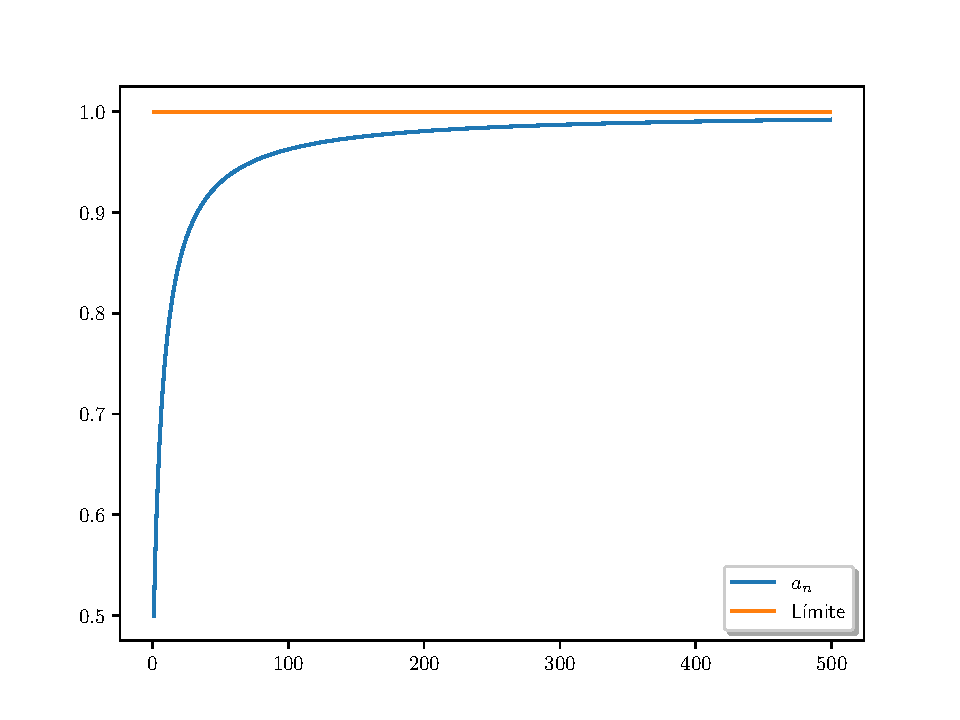
\includegraphics[width=7.5cm]{questions/p5}
        \end{figure}
    \end{minipage}
    \begin{minipage}{0.4\textwidth}
        \begin{listing}[H]
            \inputminted[
                fontsize=\scriptsize,
                breaklines,
            ]{python}{questions/p5.py}
        \end{listing}
    \end{minipage}
\end{frame}

\begin{frame}[fragile]
    \begin{solution}
        \begin{columns}
            \begin{column}{0.48\textwidth}
                \inputminted[fontsize=\tiny,firstline=3,lastline=6]{python}{questions/p5.py}

                \

                \inputminted[fontsize=\tiny,firstline=8,lastline=12]{python}{questions/p5.py}

            \end{column}
            \begin{column}{0.48\textwidth}
                \inputminted[fontsize=\tiny,firstline=14,lastline=18]{python}{questions/p5.py}
            \end{column}
        \end{columns}
    \end{solution}
\end{frame}

\begin{frame}
    \begin{solution}
        \begin{algorithm}[H]
            $A\leftarrow 1.0$\;
            $B\leftarrow 1.0$\;
            $p\leftarrow 0$\;
            \Mientras{\normalfont $\left(\left(A+1\right)-A\right)-1=0$}{
                $A\leftarrow 2\ast A$\;
                $p\leftarrow p+1$\;
                \Mientras{\normalfont $\left(\left(A+B\right)-A\right)-B\neq0$}{
                    $B\leftarrow B+1$\;
                }
            }
        \end{algorithm}
    \end{solution}
\end{frame}